\newpage
\subsection{Die Winkelfunktionen}

\hfill \break
\begin{itemize}
    \item $Sin(\alpha) = \frac{GK}{H} = \frac{GK}{1} = GK$
    \item $Cos(\alpha) = \frac{AK}{H} = \frac{AK}{1} = AK$
    \item 
    \item $Tan(\alpha) = \frac{GK}{AK} = \frac{\frac{sin(\alpha)}{cos(\alpha)}}{AK}$
\end{itemize}

\hfill \break
\begin{enumerate}
    \item Trigonometriesche Grundbeziehung = $\frac{tan(\alpha)}{1} = \frac{sin(\alpha)}{cos(\alpha)}$
    \item Pythagoras = $1 = sin(\alpha)^2 + cos(\alpha)^2$
\end{enumerate}



\hfill \break
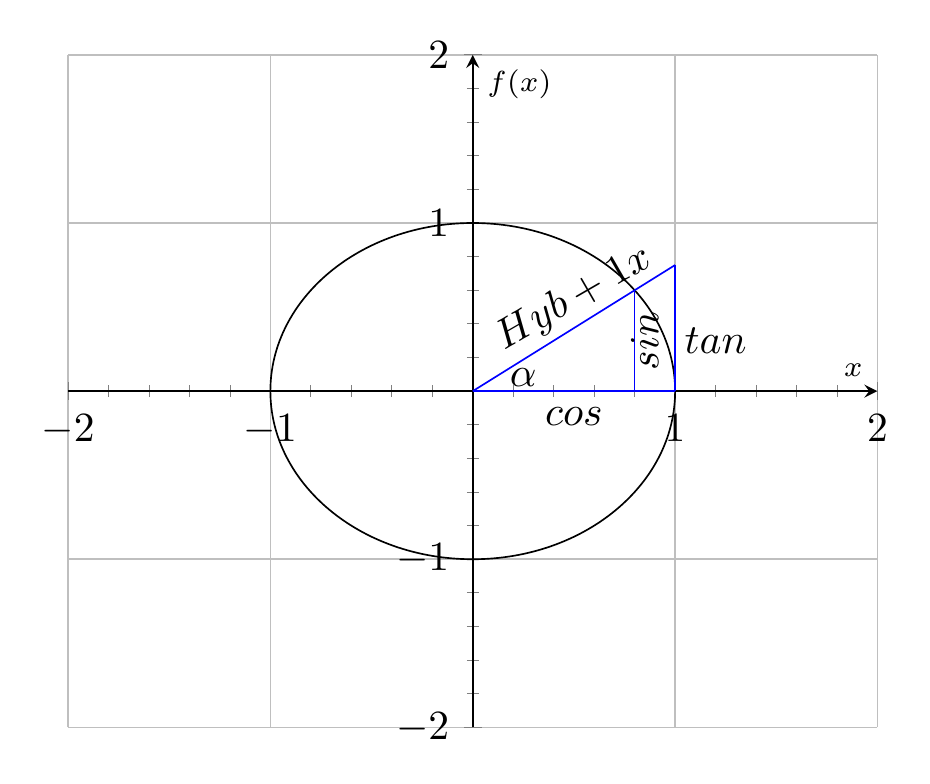
\begin{tikzpicture}[scale=1.5]
    \begin{axis}%
        [
            grid=major,
            xtick={-2,-1,...,2},
            minor x tick num=4,
            xmin=-2,
            xmax=2,
            xlabel={\scriptsize $x$},
            axis x line=middle,
            ytick={-2,-1,...,2},
            minor y tick num=4, 
            ymin=-2,
            ymax=2,
            ylabel={\scriptsize $f(x)$},
            axis y line=middle,
            no markers,
            samples=100,
            domain=-6:6,
        ]

        \draw[] (0,0) circle (1);
        \draw[color=blue] (0,0) -- (0.8,0.6);
        \draw[color=blue] (0.8,0) -- (0.8,0.6);
        \draw[color=blue] (0,0) -- (0.8,0);
        \draw[color=blue] (0.8,0.6) -- (1,0.75);
        \draw[color=blue] (1,0) -- (1,0.75);
        \draw[color=blue] (0.8,0) -- (1,0);


        \node[] at (0.25,0.08) {$\alpha$};
        \node[] at (0.5,-0.15) {$cos$};
        \node[rotate=90] at (0.85,0.3) {$sin$};
        \node[] at (1.2,0.3) {$tan$};
        \node[rotate=30] at (0.5,0.55) {$Hyb + 1x$};

    \end{axis}
\end{tikzpicture}